\section{Near-Ballistic Transfers between the Earth-Moon and Sun-Earth Systems}
While both categories of trajectories travel through the Sun-Earth CR3BP region, only those with an
intermediate staging orbit have a constrained path. For these trajectories, the Earth-Moon unstable
manifold arc, propagated under the Sun-Earth CR3BP dynamics once it reaches the lunar sphere of
influence, must intersect with a stable manifold arc from the Sun-Earth staging $L_{2}$ halo orbit.
An unstable manifold arc from this orbit is then used to depart the Sun-Earth system (compared to
the more direct transfer type that uses the Earth-Moon manifold to depart the system). Kakoi
developed a design methodology for maneuver-free transfers between orbits in the two systems,
treating them as non-coplanar, where the required respective initial orientations of the three
bodies (the Sun, Earth, and Moon) are represented by angles and the interface between the CR3BP
systems occurs at the intersection of the manifolds\cite{Kakoi:2014,Kakoi:2015}. This methodology
inspired the approach used in this investigation, where the orientations are determined by a
specified epoch date and the two systems interface before the arc intersection.

\subsection{Methodology}
To find a connection between the orbits in the two different CR3BP systems, discretized arcs of the
manifold surface of the Earth-Moon departure orbit are propagated to the SoI of the Moon, as
defined in \cref{eq:blendedSoI}. At this distance from the Moon, its gravitational influence
becomes negligible compared to those of the Earth and the Sun. At this interface of the two CR3BP
systems, the Earth-Moon barycentric rotating frame state of each arc is transformed to a Sun-Earth
barycentric rotating frame state by rotation to the Earth-centered Ecliptic J2000 inertial frame
and back as described in Section 2.5.2. This rotation depends on the epoch date when the state
reaches the SoI, as this determines the relative orientations of the celestial bodies. While the
orientations change slightly month-to-month due to the different planes, the transfer
characteristics tend to repeat each month, so this study only investigates transfers during January
2026\cite{Parker:2013}.

Note that although these states all had the same Earth-Moon Jacobi constant
value, now that they are in the Sun-Earth system, their Jacobi constant values will vary. Since
these new values will remain constant as the states are now propagated with the Sun-Earth CR3BP
equations of motion, it is necessary that the Jacobi constant of the Sun-Earth staging halo lies
within that range of values. The manifold arcs are now propagated until they reach the manifold
intersect hyperplane, chosen as an angle measured from the $x$-axis in the Sun-Earth rotating
frame. According to Kakoi, hyperplane angles between $-\ang{85}$ and $\ang{70}$ are desirable for
transfers between Earth-Moon $L_{2}$ and Sun-Earth $L_{2}$ orbits, with $\ang{-80}$ being used in
this investigation\cite{Kakoi:2015}. At the same time, the discretized stable manifold surface from
the Sun-Earth $L_{2}$ halo orbit is propagated to the same hyperplane, as shown in
\cref{fig:hyperplane}.

\begin{figure}[ht]
    \centering
    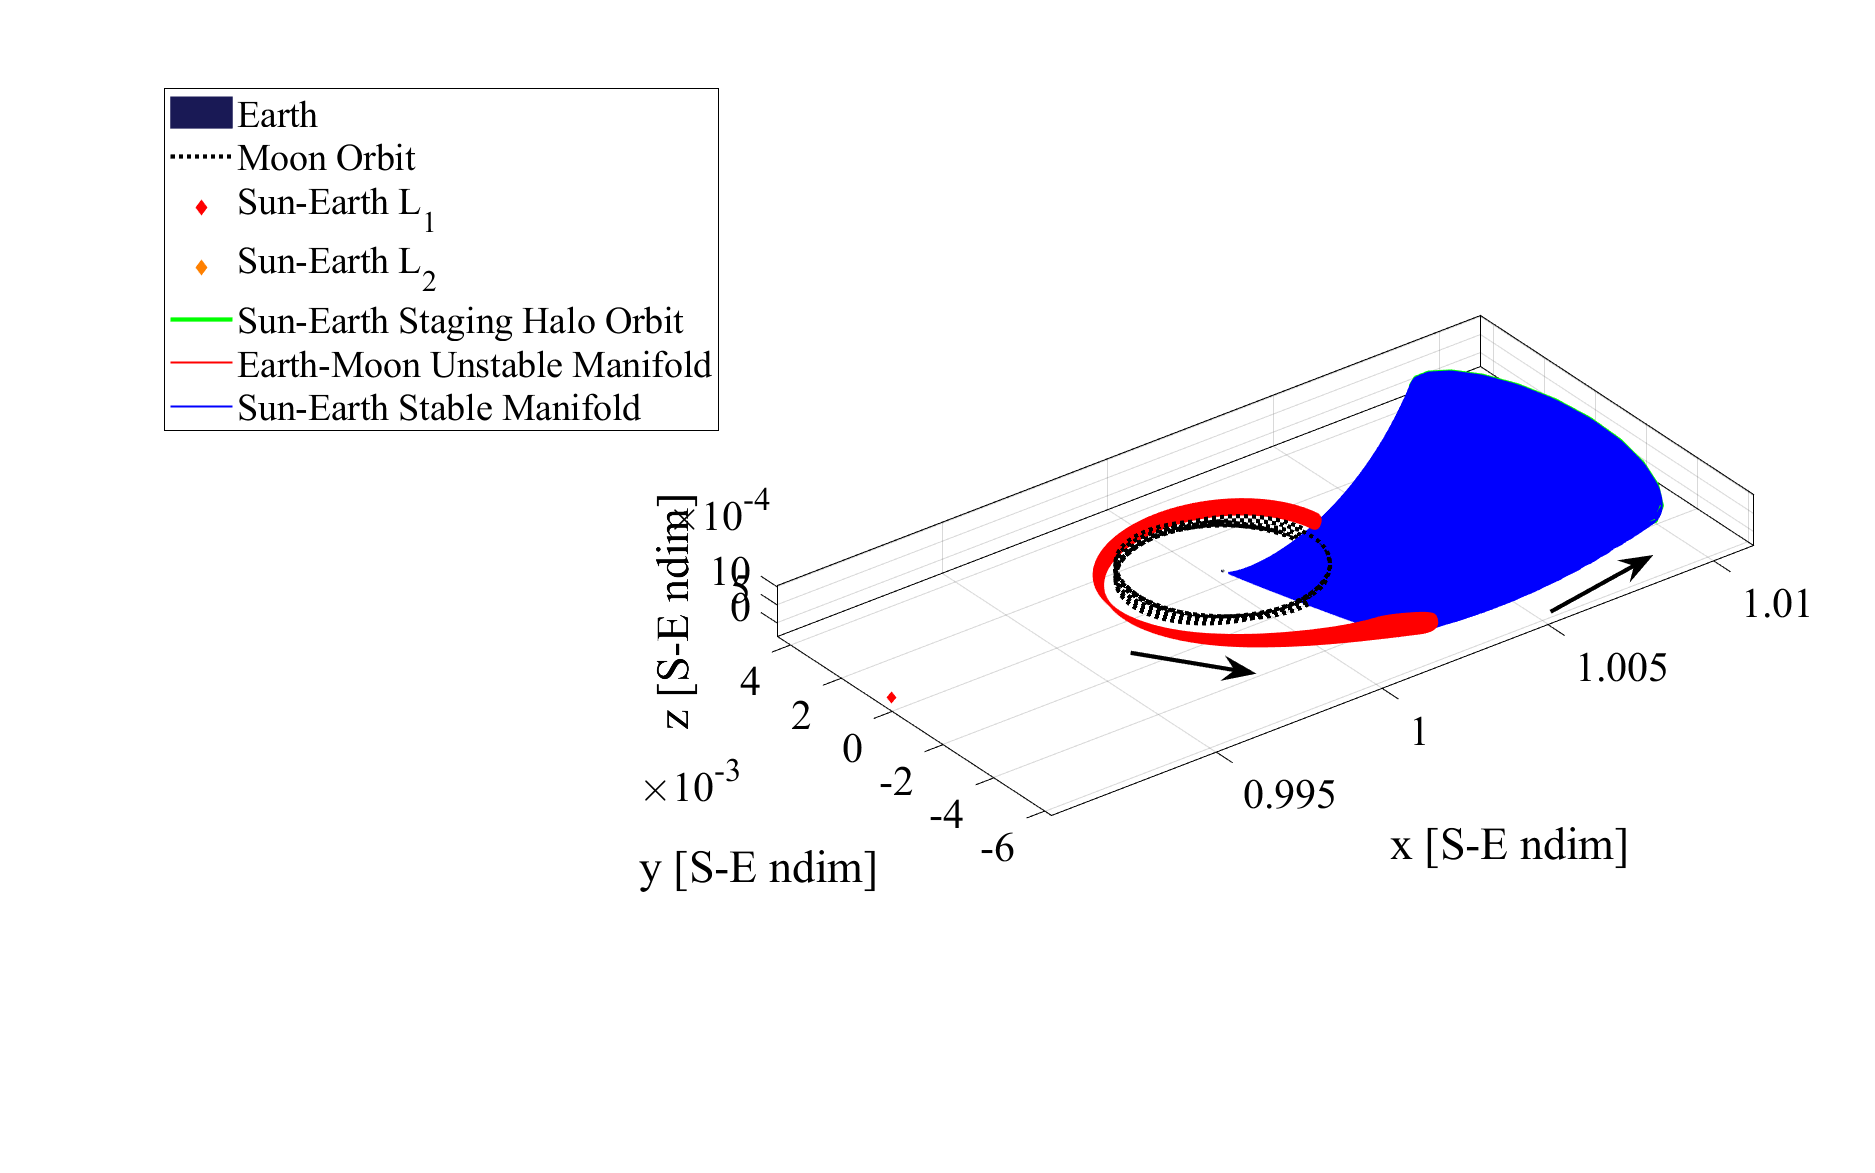
\includegraphics[width=0.9\textwidth]{figures/Hyperplane.pdf}
    \caption{Earth-Moon and Sun-Earth manifolds intersecting at the hyperplane in the Sun-Earth rotating frame.}
    \label{fig:hyperplane}
\end{figure}

At the hyperplane, mappings of both manifolds are used to form phase plots that inform the transfer
initial guess selection. Following Kakoi's approach, the plots represent $\xdot$ vs. $x$, $z$ vs.
$x$, and $\zdot$ vs. $z$. The $y$-value is defined by the $x$-value and the hyperplane angle, while
the $\ydot$-value is determined by the Jacobi constant\cite{Kakoi:2015}. A black dot along the
Earth-Moon manifold curve is also used to denote the arc that matches the Sun-Earth manifold in
Jacobi constant. The two sets of manifold arcs form curves on the plots and the goal is to find an
intersection between the curves in all three phase plots that occurs at the black point.
\cref{fig:phasePlots} shows an example of these phase plots, where the red curve is the unstable
Earth-Moon manifold and the blue curve is the stable Sun-Earth manifold. Note that there are two
black markers representing two arcs that match the Sun-Earth Jacobi constant.

\begin{figure}[ht]
    \centering
    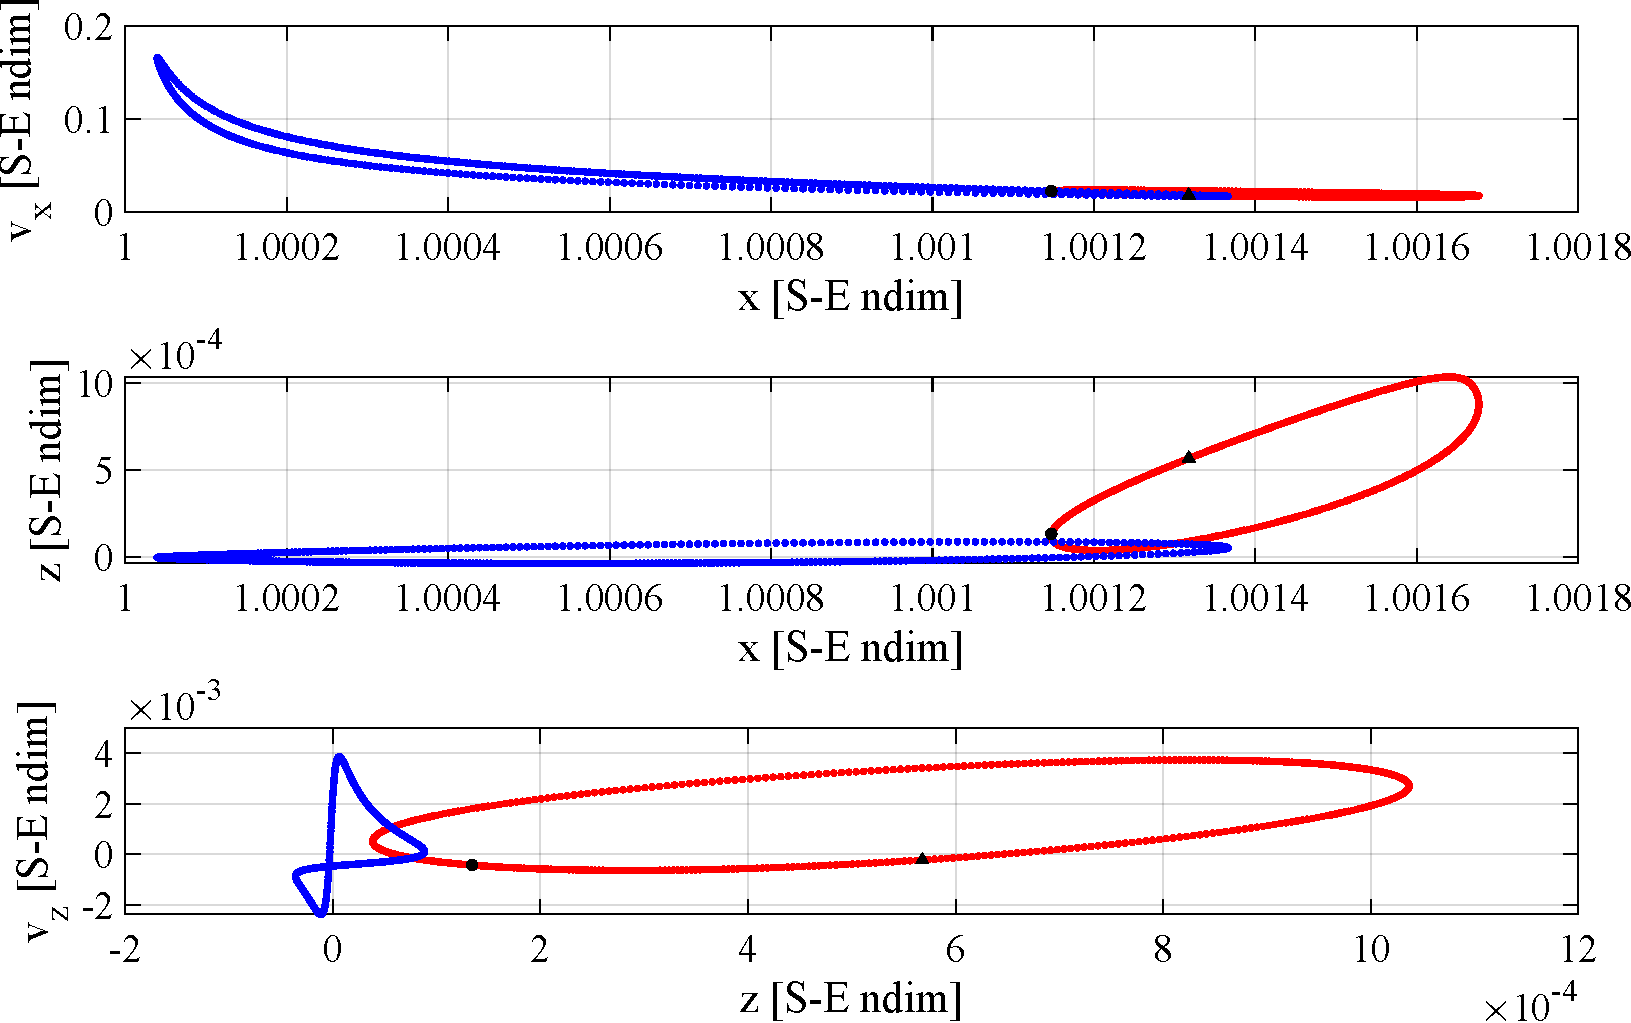
\includegraphics[width=0.75\textwidth]{figures/PhasePlots.pdf}
    \caption{The hyperplane phase plots for \cref{fig:hyperplane}.}
    \label{fig:phasePlots}
\end{figure}

The initial epoch of the Earth-Moon manifold departure, the hyperplane angle, and the Sun-Earth
halo Jacobi constant can all be varied to shift the curves on the phase plots and find an
intersection; Kakoi provides some guidelines on how to do so\cite{Kakoi:2015}. Once a suitable
point is determined, like the black circle marker in \cref{fig:phasePlotsIntersect}, this
information can be used to generate an initial guess for the transfer between the systems, which is
shown in \cref{fig:initialGuess}.

\begin{figure}[ht]
    \centering
    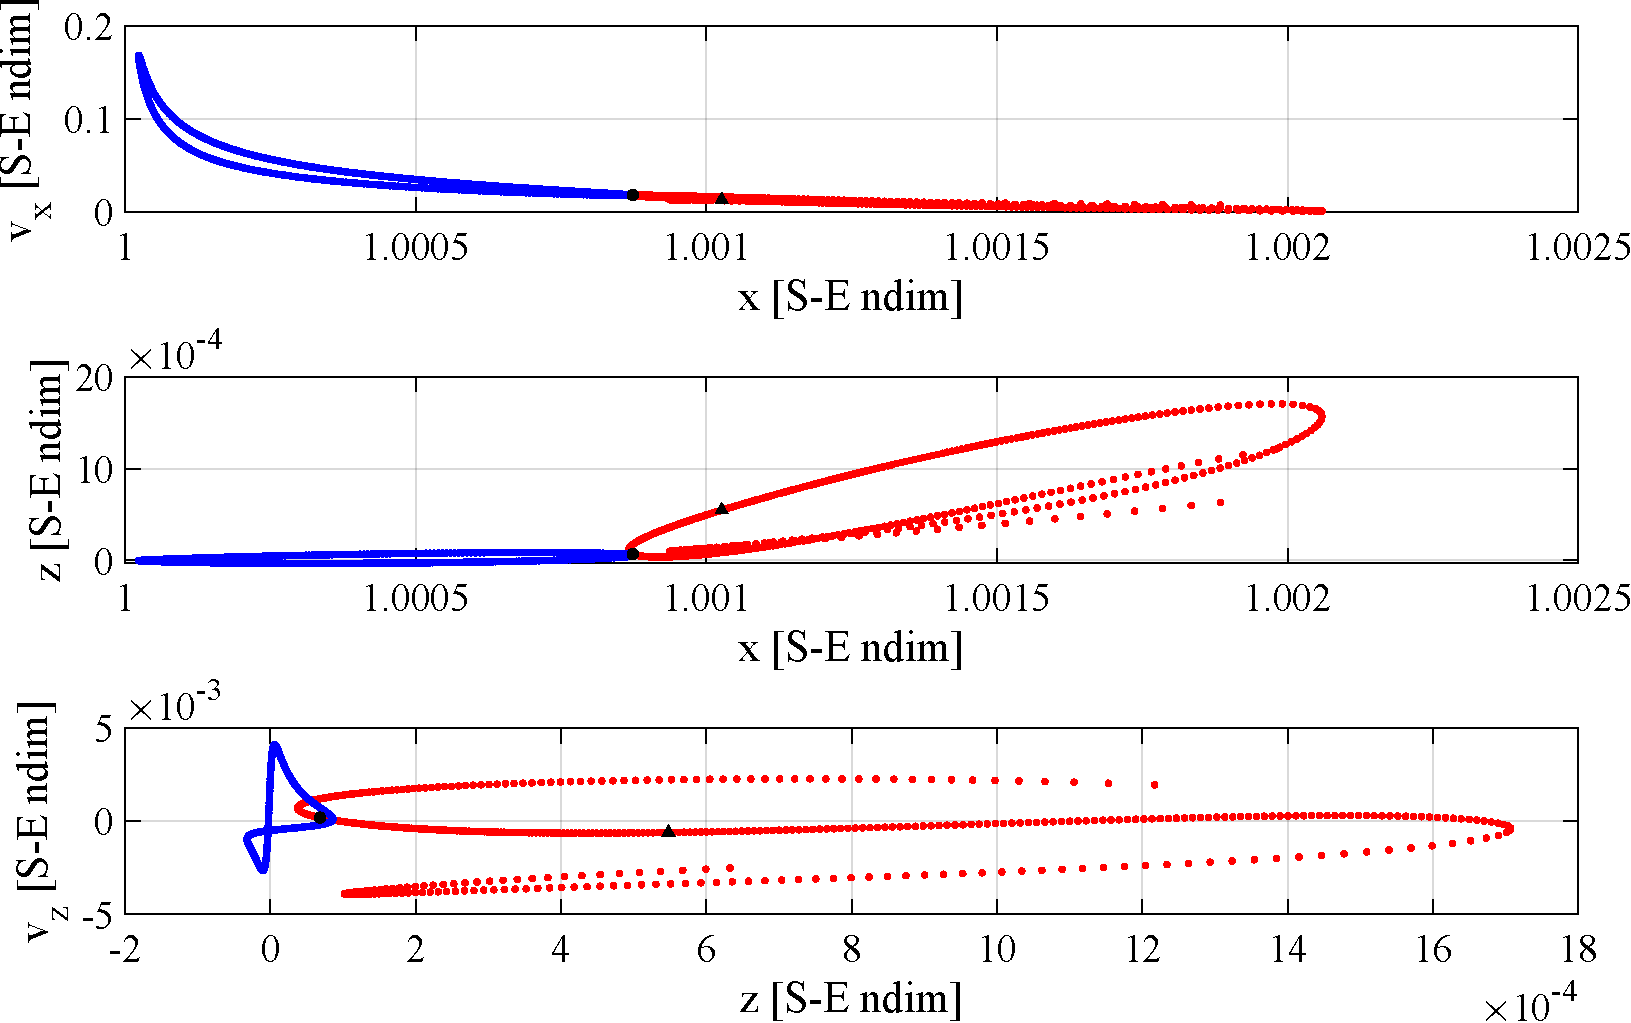
\includegraphics[width=0.75\textwidth]{figures/PhasePlotsIntersect.pdf}
    \caption{Hyperplane phase plots with a near intersection after varying the parameters.}
    \label{fig:phasePlotsIntersect}
\end{figure}

\begin{figure}[ht]
    \centering
    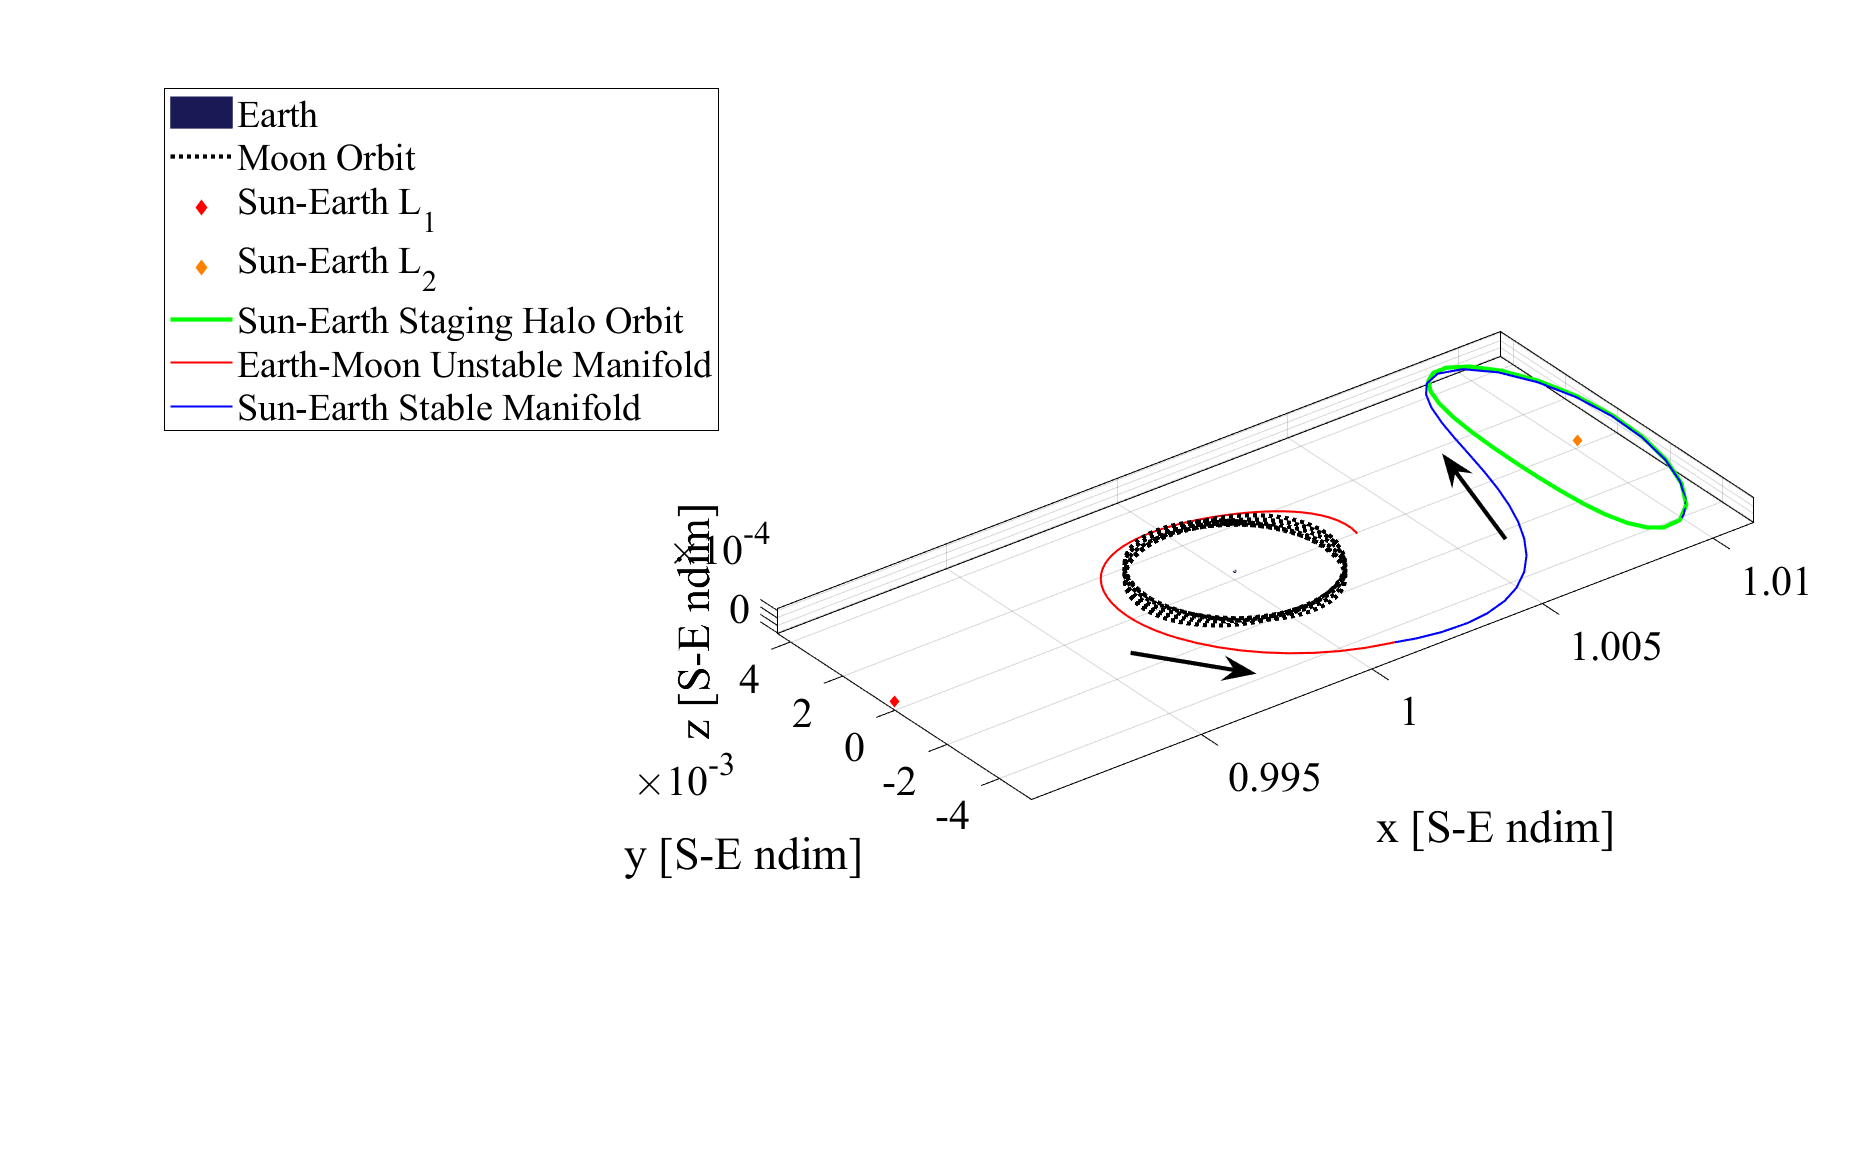
\includegraphics[width=0.9\textwidth]{figures/InitialGuess.pdf}
    \caption{Initial guess for near-ballistic Earth-Moon to Sun-Earth transfer using phase plots in the Sun-Earth rotating frame.}
    \label{fig:initialGuess}
\end{figure}

This initial guess is then corrected to find a position intersection (a maneuver is allowed at the
intersection) using an iterative Newton-Raphson scheme:
\begin{equation}
    \Xbar=\begin{bmatrix}   T_{0}   &   \tau_{1}    &   t_{1}   &   \tau_{2}    &   t_{2}   \end{bmatrix}^{T},
    \label{eq:nbfreevar}
\end{equation}
\begin{equation}
    \Fbar(\Xbar)=\begin{bmatrix}    \rbar_{2}-\rbar_{1} &   ||\vbar_{2}-\vbar_{1}|| \end{bmatrix}^{T}.
    \label{eq:nbconst}
\end{equation}
where $T_{0}$ is the initial epoch, $\tau_{1}$ and $\tau_{2}$ are the phase along the Earth-Moon
and Sun-Earth orbits, respectively, where the manifold steps-off, $t_{1}$ and $t_{2}$ are the
times-of-flight along each manifold arc, respectively, $\rbar_{1}$ and $\rbar_{2}$ are the manifold
arc positions at the end of the propagation, and $\vbar_{1}$ and $\vbar_{2}$ are the velocity
vectors at those points. The central difference method from Section 3.1.3 is used to determine the
$DF$ Jacobian matrix. Note that the magnitude of the maneuver is included as the second constraint
in the targeting problem. For the first implementation of the targeter, the $\Delta v$ of the
initial guess is used as the constraint. Then, each time a solution is converged, this constraint
value is decreased and the targeting problem is repeated to find a near-ballistic solution with a
local minimum in $\Delta v$. Also note that during this process, the intersection location of the
two manifold arcs is free to shift from the designated hyperplane. The result of this process is a
near-ballistic transfer between an Earth-Moon orbit and a Sun-Earth halo orbit utilizing their
invariant manifolds. These transfers have low enough maneuver costs that will likely be rendered
negligible once the solution is transferred to a higher-fidelity dynamical model.

\subsection{Example}
As an example, consider the phase plots in \cref{fig:phasePlotsIntersect} and the resulting initial
guess in \cref{fig:initialGuess}. The unstable manifold arc departs from an Earth-Moon northern
halo orbit with an Earth-Moon Jacobi constant of $3.13$ on January 2, 2026 at 07:12:00, while the
stable manifold arc arrives at a Sun-Earth northern halo orbit with a Sun-Earth Jacobi constant of
$3.0008189$. At the hyperplane intersection, these two arcs have a position discontinuity of
$8.768\times10^{-6}$ Sun-Earth nondimensional units ($1312$ km) and a $\Delta v$ of $57.4$ m/s. The
iterative corrections process outlined above produces a position continuous trajectory with a
$\Delta v$ of $14.6$ m/s, a negligible amount in comparison to the rest of the end-to-end transfer.
The initial departure epoch has also shifted slightly, to January 2, 2026 at 07:32:35. This
corrected trajectory is shown in \cref{fig:solution}. Note that the location of the maneuver has
shifted from the defined hyperplane to earlier along the Earth-Moon manifold arc. While this exact
solution is only available for the given epoch, every month a similar solution presents itself, so
this one can be used to represent the potential near-ballistic transfer solutions.

\begin{figure}[ht]
    \centering
    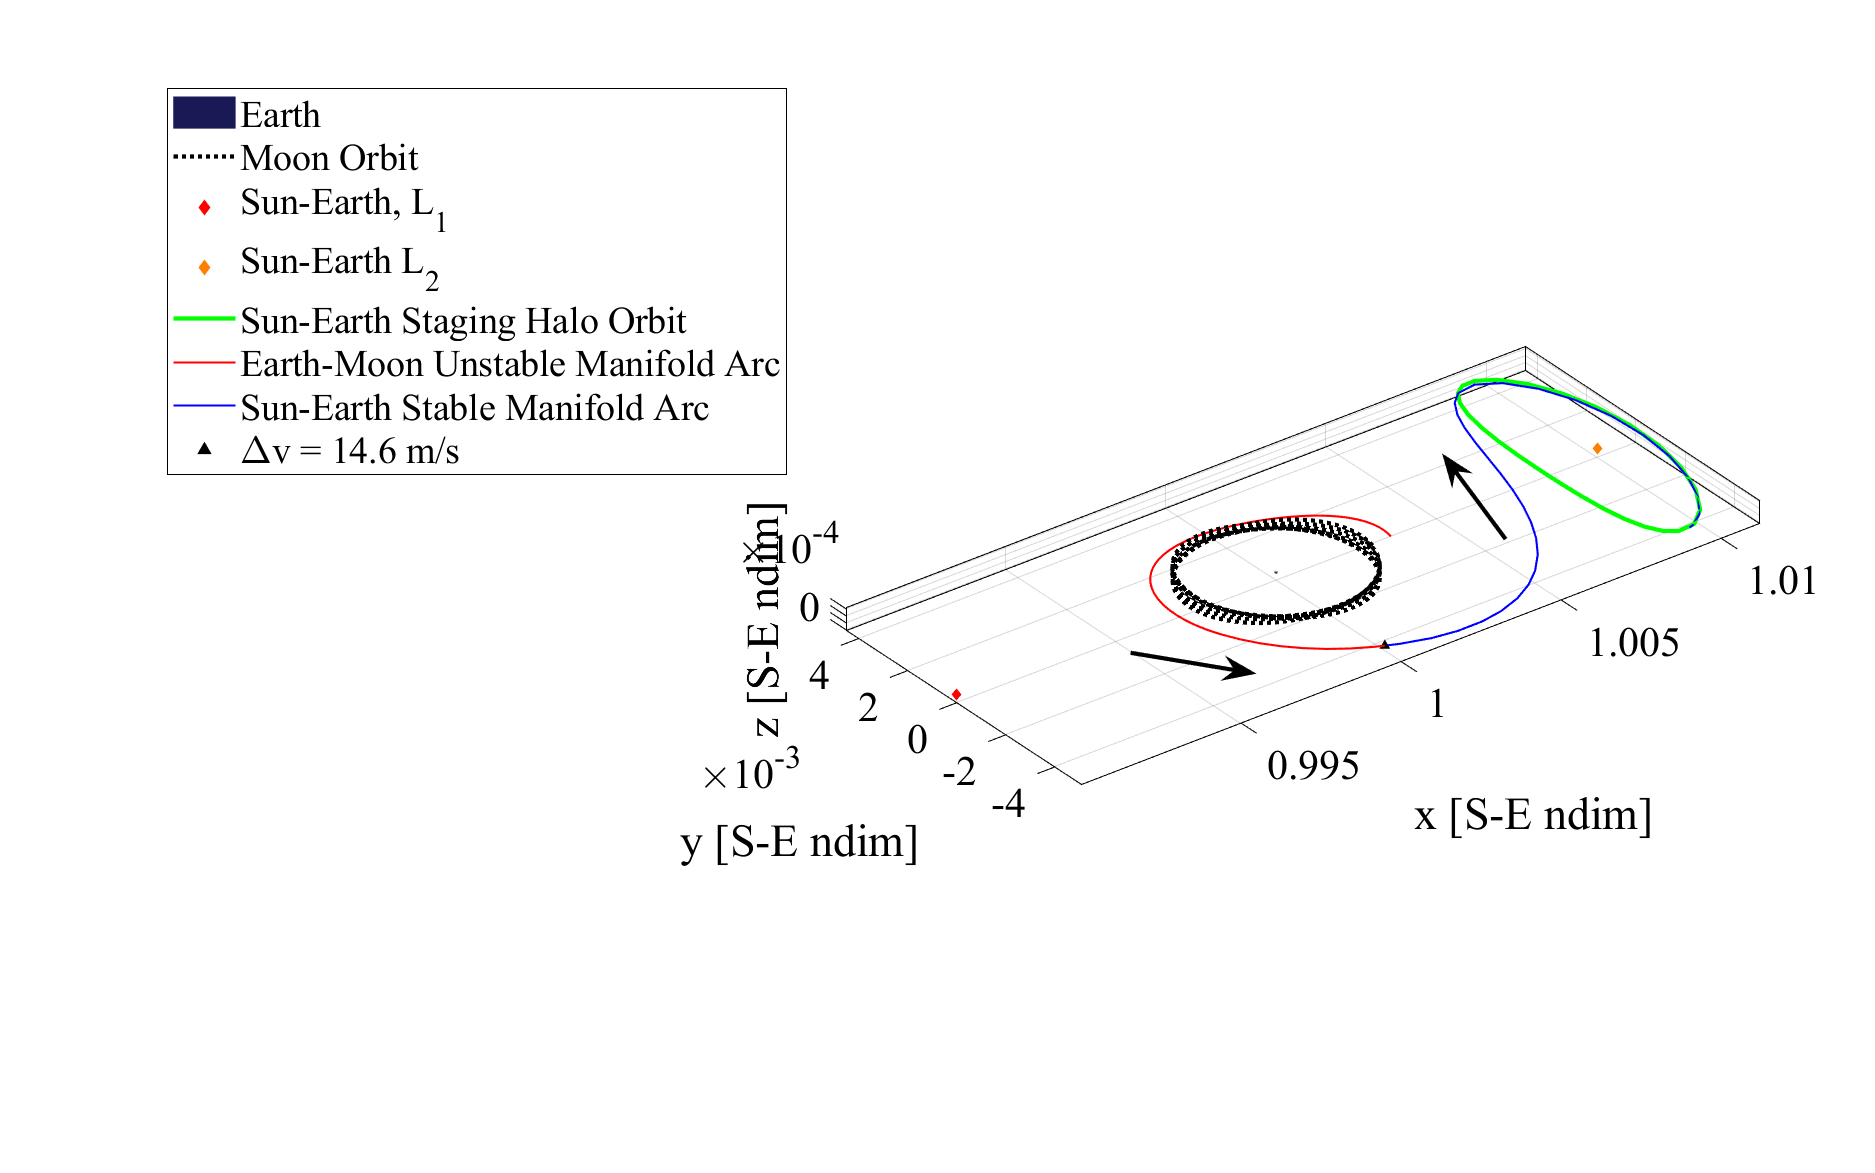
\includegraphics[width=0.9\textwidth]{figures/Solution.pdf}
    \caption{Converged near-ballistic tranfer between Earth-Moon and Sun-Earth halo orbits in the Sun-Earth rotating frame.}
    \label{fig:solution}
\end{figure}
